\documentclass[main.tex,fontsize=8pt,paper=a4,paper=portrait,DIV=calc,]{scrartcl}
% Document
\usepackage[T1]{fontenc}
\usepackage[dvipsnames]{xcolor}
\usepackage[nswissgerman,english]{babel}
\renewcommand{\familydefault}{\sfdefault}

% Format
\usepackage[top=5mm,bottom=1mm,left=5mm,right=5mm]{geometry}
%\setlength{\headheight}{\baselineskip}
%\setlength{\headsep}{0mm}

%\usepackage{scrlayer-scrpage}
%\clearpairofpagestyles
%\chead{{\bfseries\TITLE, \AUTHOR, \pagename~\thepage}}

%\addtokomafont{pagehead}{\upshape}

\usepackage{multicol}
\setlength{\columnsep}{2mm}
\setlength{\columnseprule}{0.1pt}

% Math
\usepackage{amsmath}
\usepackage{amssymb}
\usepackage{amsfonts}

% Code
\usepackage{fancyvrb, etoolbox, listings, xcolor}
%\usemintedstyle{bw}

%\newminted[shell]{bash}{
%fontsize=\footnotesize,
%fontfamily=tt,
%breaklines=true,
%frame=single,
%framerule=0.1pt,
%framesep=2mm,
%tabsize=2
%}
%\newminted{css}{
%breaklines=true,
%tabsize=4,
%autogobble=true,
%escapeinside=||,
%stripall=true,
%stripnl=true,
%}

    \definecolor{lightgray}{rgb}{0.95, 0.95, 0.95}
    \definecolor{darkgray}{rgb}{0.4, 0.4, 0.4}
    \definecolor{purple}{rgb}{0.65, 0.12, 0.82}
    \definecolor{ocherCode}{rgb}{1, 0.5, 0} % #FF7F00 -> rgb(239, 169, 0)
    \definecolor{blueCode}{rgb}{0, 0, 0.93} % #0000EE -> rgb(0, 0, 238)
    \definecolor{greenCode}{rgb}{0, 0.6, 0} % #009900 -> rgb(0, 153, 0)
    \definecolor{teal}{rgb}{0.0, 0.5, 0.5}

\lstdefinestyle{code}{
    identifierstyle=\color{black},
    keywordstyle=\color{blue}\bfseries\small,
    ndkeywordstyle=\color{greenCode}\bfseries\small,
    stringstyle=\color{ocherCode}\ttfamily\small,
    commentstyle=\color{teal}\ttfamily\textit\small,
    basicstyle=\ttfamily\small,
    breakatwhitespace=false,         
    breaklines=true,                 
    captionpos=b,                    
    keepspaces=true,                 
    showspaces=false,                
    showstringspaces=false,
    showtabs=false,                  
    tabsize=2,
    belowskip=-5pt
}



% Images
\usepackage{graphicx}
\newcommand{\pic}{\includegraphics[scale=0.3]}
\graphicspath{{Screenshots/}{../Screenshots}}
\makeatletter
\def\pictext#1#2{%
    \@ifnextchar[{%
    \pictext@iiiii{#1}{#2}%
    }{%
      \pictext@iiiii{#1}{#2}[0.5,0.4,0.3]% Default is 5
    }%
}
\def\pictext@iiiii#1#2[#3,#4,#5]{\begin{minipage}{#3\textwidth}\includegraphics[scale=#4]{#1}\end{minipage}\begin{minipage}{#5\textwidth}#2\end{minipage}}
\def\minipg#1#2{%
    \@ifnextchar[{%
    \minipg@iiii{#1}{#2}%
    }{%
      \minipg@iiii{#1}{#2}[0.3,0.6]% Default is 5
    }%
}
\def\minipg@iiii#1#2[#3,#4]{\vspace{0.8mm}\begin{minipage}{#3\textwidth}#1\end{minipage}\begin{minipage}{#4\textwidth}#2\end{minipage}{\vspace{0.8mm}}}
\makeatother

%\newenvironment{minty}[2]% environment name
%{% begin code
%  \begin{minipage}{#1}
%  \begin{minted}{#2}
%}%
%{% end code
%  \end{minted}
%  \end{minipage}
%  \end{minty}\ignorespacesafterend
%} 

% Smaller Lists
\usepackage{enumitem}
\setlist[itemize,enumerate]{leftmargin=3mm, labelindent=0mm, labelwidth=1mm, labelsep=1mm, nosep}
\setlist[description]{leftmargin=0mm, nosep}
\setlength{\parindent}{0cm}

% Smaller Titles
\usepackage[explicit]{titlesec}

%% Color Boxes
\newcommand{\sectioncolor}[1]{\colorbox{black!60}{\parbox{0.989\linewidth}{\color{white}#1}}}
\newcommand{\subsectioncolor}[1]{\colorbox{black!50}{\parbox{0.989\linewidth}{\color{white}#1}}}
\newcommand{\subsubsectioncolor}[1]{\colorbox{black!40}{\parbox{0.989\linewidth}{\color{white}#1}}}
\newcommand{\paragraphcolor}[1]{\colorbox{black!30}{\parbox{0.989\linewidth}{\color{white}#1}}}
\newcommand{\subparagraphcolor}[1]{\colorbox{black!20}{\parbox{0.989\linewidth}{\color{white}#1}}}

%% Title Format
\titleformat{\section}{\vspace{0.5mm}\bfseries}{}{0mm}{\sectioncolor{\thesection~#1}}[{\vspace{0.5mm}}]
\titleformat{\subsection}{\vspace{0.5mm}\bfseries}{}{0mm}{\subsectioncolor{\thesubsection~#1}}[{\vspace{0.5mm}}]
\titleformat{\subsubsection}{\vspace{0.5mm}\bfseries}{}{0mm}{\subsubsectioncolor{\thesubsubsection~#1}}[{\vspace{0.5mm}}]
\titleformat{\paragraph}{\vspace{0.5mm}\bfseries}{}{0mm}{\paragraphcolor{\theparagraph~#1}}[{\vspace{0.5mm}}]
\titleformat{\subparagraph}{\vspace{0.5mm}\bfseries}{}{0mm}{\subparagraphcolor{\thesubparagraph~#1}}[{\vspace{0.5mm}}]

%% Title Spacing
\titlespacing{\section}{0mm}{0mm}{0mm}
\titlespacing{\subsection}{0mm}{0mm}{0mm}
\titlespacing{\subsubsection}{0mm}{0mm}{0mm}
\titlespacing{\paragraph}{0mm}{0mm}{0mm}
\titlespacing{\subparagraph}{0mm}{0mm}{0mm}

%% format cells
\usepackage[document]{ragged2e}
\usepackage{array, makecell}
\renewcommand{\arraystretch}{2}
\newcommand{\mc}{\makecell[{{m{1\linewidth}}}]}


\begin{document}
\begin{table}[h!]
\section{Terms and Definitions}
\begin{tabular}{|m{0.2\linewidth}|m{0.755\linewidth}|}
\hline
AGI Articifial General Intelligence & This is the hypothetical goal of achieving an AI that can perform general task as good or even better than a human. Aka, the goal is to essentially mimic a human in their general life. \\
\hline
Turing test & This is an idea that if a machine can do X task just like a human, aka indistinguishable from the human, then the machine has passed the Turing test. The problem with this however, is that a machine needs to learn to lie, since a human can do this as well -> see the pinoccio problem. The second problem is that certain tasks are too complex for humans but might not be for a machine, in this case the Turing test simply makes no sense. \\
\hline
Machine Learning & Machine Learning is comprised of 3 different techniques. Supervised learning, unsupervised learning and reinforcement learning. Supervised and unsupervised are not that different other tan the presence of the human. Reinforcement learning however is different as the AI is rewarded for "good" behavior/results and "punished" for bad behavior/results. \\
\hline
NLP Natural Language Processing & The research field of trying to achieve both understanding and creation of natural human language by AI. While development has been in the works for quite a while, because AI can't understand context, it is still very much "in beta". \\
\hline
\emph{The 4 Ingredients of Machine-Learning} & 
\vspace{2mm}
\begin{enumerate}
\item Data \newline
In order for a machine to learn anything you need to provide it with data to work with.
\item Cost-Function(Loss) \newline
You need a way to tell your machine what is considered to be good or bad. \newline
Without it the machine can't learn from it's previous endeavors.\newline
\item Model \newline
This can be something simple as 2 parameters like \(y_i = ax_i + b\) or something complicated like a neural network.\newline
We usually use something like \emph{tensorflow} or \emph{pytorch} to define the model\newline
At the end of the day it is always some sort of \textbf{mathematical function!}
\item Optimization
An algorithm that minimizes the amount of parameters needed for the cost function. \newline
Usually something like Stochastic Gradient Descent(SGD), ADAM, RMSProp 
\end{enumerate}
\vspace{2mm}
There are many more, but these 4 are the most important. You might also care about performance optimization\newline
visualization and validation though.\\
\hline
\end{tabular}
\subsection{Representation of words}
\begin{tabular}{|m{0.2\linewidth}|m{0.755\linewidth}|}
\hline
\textbf{\emph{One-hot vector}} & \minipg{ 
This is a vector with 1 value set to 1, this represents the word.\newline
If you now iterate over a sentence, you will end up with a matrix.\newline}
{\pic{2022-09-29:08:51:08.png}}[0.3,0.7]\newline
Problems with this approach\newline
\begin{itemize}
\item high dimensionality\newline
for 100,000 words you would need 100,000 dimensions to the vector.\newline
\item sparse information\newline
The vast majority of the vector aka all but one, is just 0's, this is not data!.\newline
\item no generalization \newline
There is no context for words, no groups, no terms.\newline
For example a car is associated with tires but not with mangos.\newline
This method can't associate anything with anything.\newline
\end{itemize}
\\
\hline
\textbf{\emph{Indexing}} & 
Indexing simply assigns a number to a word. \newline
This approach solves the problem of having a vector with mostly 0's,\newline
but it does not solve the problem of not having context, a mango still has no boundary.\\
\hline
\textbf{\emph{Distributed Representation (dense vectors)}} & \minipg{
This finally solves the issue of context to a certain extend.\newline
We represent a context with a color, if 2 words have the same color in their graph, then there is overlap with these words.\newline
In the following figure the context male is represented in the words man and king, while the context female is represented in the words queen and woman.}
{\pic{2022-09-29:09:14:13.png}}[0.4,0.4]\newline
\minipg{
The way this is done is with a vector that is dense,\newline
this means that this vector has data in multiple dimensions to show context.
}{\pic{2022-09-29:09:19:18.png}}[0.28,0.4]\newline
Important other things to remember:\newline
\begin{itemize}
\item The dot product of 2 vectors becomes 1 if the vectors are parallel.
\item The dot product of 2 vectors becomes 0 if the vectors are orthogonal -> 90 degree angle.
\item The dot product of 2 vectors becomes -1 if the vectors are in the opposite direction.
\end{itemize}\\
\hline
\end{tabular}
\end{table}
\pagebreak
\begin{table}[h!]
\begin{tabular}{|m{0.2\linewidth}|m{0.755\linewidth}|}
\hline
\textbf{\emph{Distance between word vectors}} &
\minipg{
Just like with a regular vector you can calculate the distance between a vector.\newline
Similarly you can also calculate the angle between 2 vectors instead.\newline
}{\pic{2022-09-29:09:34:08.png}}[0.28,0.6]\\
\hline
\textbf{\emph{Finding vector representations}} & 
The obvious question is how do we get the representation of vectors?\newline
\begin{itemize}
\item The first way is to simply use pretrained models that already have the vectors.\newline
\item The other way is to use an embedding layer, this can be done with tools like \textbf{\emph{word2vec}}.\newline
With word2vec you can also use predefined embeddings in order to save you some work.\newline
Another one of these embeddings is \textbf{\emph{GloVe}}.
\end{itemize}
Important tool for creating classes for embedding layers: \textcolor{red}{\textbf{\emph{Keras}}}\\
\hline
\end{tabular}
\subsection{Random Variables}
\begin{tabular}{|m{0.2\linewidth}|m{0.755\linewidth}|}
\hline
\textbf{Discrete and continuous} & \minipg{
Discrete variables are a set of finite numbers.\newline
\large \( X = { 1.5 , 2.678 , 5 , 6.3 , 10 } \)\newline}
{\pic{2022-10-06:08:25:05.png}}[0.3,0.4]\newline
\minipg{
\normalsize Continuous variables are a range of numbers.\newline
\large \( X = (2, 7 ) \) 2 to 7\newline\normalsize}
{\pic{2022-10-06:08:25:08.png}}[0.3,0.4]\\
\hline
Likelyhood and Base information &
The maximum amount of information we can have about a random variable is \textbf{the possible value it can have}, see the set above.\newline
And \textbf{the likelyhood of a specific value appearing}.\\
\hline
\textbf{Notations} & \minipg{
  \emph{\textcolor{teal}{Pr(X=x) is often written in the more compact form P(x) or p(x), or sometimes as PX(x) (there's no formal rule)}}}
{\pic{2022-10-06:08:38:46.png}}[0.3,0.5]\\
\hline
Dice example &
\pic{2022-10-06:08:49:14.png} \pic{2022-10-06:08:49:26.png}\\
\hline
\textbf{Probability Mass Function (PMF)} &
\pic{2022-10-06:08:51:23.png} \pic{2022-10-06:08:52:19.png}\\
\hline
\textbf{Joint Probability} & 
Joint probability is simply the probability of more than 1 thing, in this case 2.\newline
\textcolor{red}{\textbf{If the variables are dependent on each other:}}\newline
\huge \( Pr(A,B) = Pr( A \text{ given } B) * Pr(B) \)\newline
\normalsize \textcolor{teal}{We multiply the chance of A \textbf{(considering A and B can be true at the same time)} with the chance of B.}\newline
For example \(Pr(A \text{ given }B) = 0 \), this means A can't happen when B happens.\newline
\textcolor{red}{\textbf{If the variables are \emph{NOT} dependent on each other:}}\newline
\huge \( Pr(A,B) = Pr(A) * Pr(B) \)\newline
\normalsize \textcolor{teal}{We multiply the chance of A with the chance of B. (independent of each other)}\\
\hline
\textbf{Conditional Probability} & 
This is the \textbf{opposite of Joint Probability with dependence}.\newline
\huge \( P(X,Y) = P(X | Y) P(Y) \)\newline
\normalsize\textcolor{teal}{This is the probability of x and y if y is true. aka probability of x if y is true * probability of y}\\
\hline
\textbf{Bayes Rule} & \minipg{
  Bayes rule uses the fact that we can substitute variables,\newline 
  here we substitute the conditional probability of 2 variables.\newline
  \pic{2022-10-06:09:44:53.png}
}
{\pic{2022-10-06:09:18:12.png}}[0.4,0.4]
\\
\hline
\end{tabular}
\end{table}
\pagebreak
\begin{table}[ht!]
\begin{tabular}{|m{0.2\linewidth}|m{0.755\linewidth}|}
\hline
Confusion Matrix & 
This is simply a matrix that shows correlation of 2 things in a row.\newline
Theoretically, since they are dependent, they should only provide either both true or both false.\newline
However, this is not always the case.\newline
\textcolor{orange}{The general rule: True Positives and True Negatives should always be higher than the other 2!}\newline
\pic{2022-10-20:08:33:25.png}\\
\hline
\end{tabular}
\section{Linear Regression}
\begin{tabular}{|m{0.2\linewidth}|m{0.755\linewidth}|}
\hline
Idea & 
\textcolor{teal}{The basic idea of linear regression is to check for correlation between two sets of data, for example, what is the correlation of mouse size to mouse weight? \newline
Linear regression tries to do this with a simple straight line! It is therefore the easiest way to get a correlation, but it is also not very accurate.\newline
To rectify the bad accuracy, we do this multiple times for a small sets of data, aka for slices of the data.}\\
\hline
Formula and Mean Squared Error & 
\large \(\hat{y}_i = m * x_i + d \)\newline
\( e_i = y_i - \hat{y}_i \)\newline
\huge \( E = \dfrac{1}{2N} \sum_{i=1}^{N}e_{i}^{2} \) \newline
\( MSE = \dfrac{1}{2N} \sum_{i=1}^{N}(y_i - (m * x_i +b))^2 \)\newline 
\normalsize \, \newline
Legend: \newline
\minipg{
\begin{itemize}
  \item \textcolor{orange}{m = \textbf{slope}}
\item \textcolor{orange}{\(x_i\) = x of datapoint}
\item \textcolor{orange}{\(y_i\) = y of datapoint}
\item \textcolor{orange}{\( \delta y_i \) = y of line -> mean(y)}
\item \textcolor{orange}{d = y offset / \textbf{intercept}}
\item \textcolor{orange}{\(e_i\) = single residual -> value of a datapoint}
\item \textcolor{orange}{E = sum of residuals}
\item \textcolor{orange}{N = amount of datapoints}
\vspace{-3mm}
\end{itemize}
}{
  \textcolor{red}{The \( y_i \) inside the MSE is the actual data that we have from our dataset.\newline
  While the \(m * x_i + b\) is the formula that we used. -> linear or polynomial regression.\newline
We are essentially comparing the 2 y's, the one from the data and the one from the calculation.\newline
We then square the difference and do this for every point in the dataset.\newline
Our final calculation will be the \textbf{Mean Squared Error}}
}[0.33,0.4]
\, \newline
\pic{2022-10-27:09:04:09.png}\newline
\textcolor{orange}{You need to first decide what the line is for yourself, this means manual fitting!\newline
Then you can see the Residual Error which would be \textbf{E} in the formula!}\newline
\textcolor{red}{The ultimate goal is to \textbf{MINIMIZE E -> MINIMIZE ERROR!}}\newline
\textcolor{orange}{To do this, we calculate the mean squared error by checking the difference between the data we calculated and our training data.\newline
aka the sum of (training y - calculation y) squared.}
\\
\hline
Least Squares &
\textcolor{orange}{This term simply explains the improvement of fitting a function by calculating them via derivates of slopes:}\newline
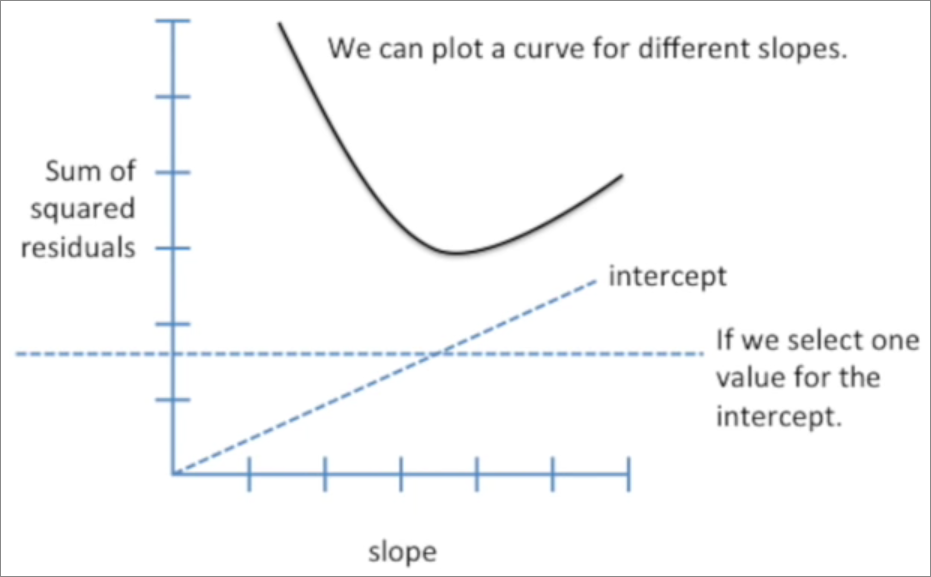
\includegraphics[scale=0.2]{2022-11-10:04:16:23.png}\newline
\textcolor{purple}{As you can see you take the derivate of MSE and slope with respect to slope and try to find a 0 value -> a local minimum or maximum.\newline
And considering we didn't use a fucked up line in the first place, we can be sure that it is indeed a \textbf{local minimum}!}\newline
\minipg{
\textcolor{OliveGreen}{\( \text{derivate in relation to slope} = \dfrac{1}{2N} \sum_{i=1}^{N} \dfrac{d}{dm}(y_i - (m * x_i +b))^2 \)}\newline 
\textcolor{OliveGreen}{\( \text{derivate in relation to slope} = \dfrac{1}{2N} \sum_{i=1}^{N} (2b (bx - y)) \)}\newline 
\textcolor{OliveGreen}{\( \text{derivate in relation to intercept} = \dfrac{1}{2N} \sum_{i=1}^{N} \dfrac{d}{db}(y_i - (m * x_i +b))^2 \)}\newline 
\textcolor{OliveGreen}{\( \text{derivate in relation to intercept} = \dfrac{1}{2N} \sum_{i=1}^{N} 2(x-y+b) \)}
}{
  \textcolor{red}{Now we need to make sure that the derivate is 0! \newline
  \( \text{MSE'} = 0 \)\newline
If this is given, then we have our slope or intercept that will fit best with our current data!}\\
}[0.44,0.31]\\
\hline
\end{tabular}
\end{table}
\pagebreak
\begin{table}[ht!]
\begin{tabular}{|m{0.2\linewidth}|m{0.755\linewidth}|}
\hline
Correlation and Causation &
\textcolor{orange}{Just because something has a mathematical correlation, does not mean that it also has a causality. Some things might be correlated for random reasons, or even simple chance. \newline
For example you might find that the increase in cats is correlated with stormy weather, the data reflects that, but if you know how the weather works, you know that this is utter bs and will never be true.}\\
\hline
Parson Correlation Coefficient & 
\vspace{2mm}
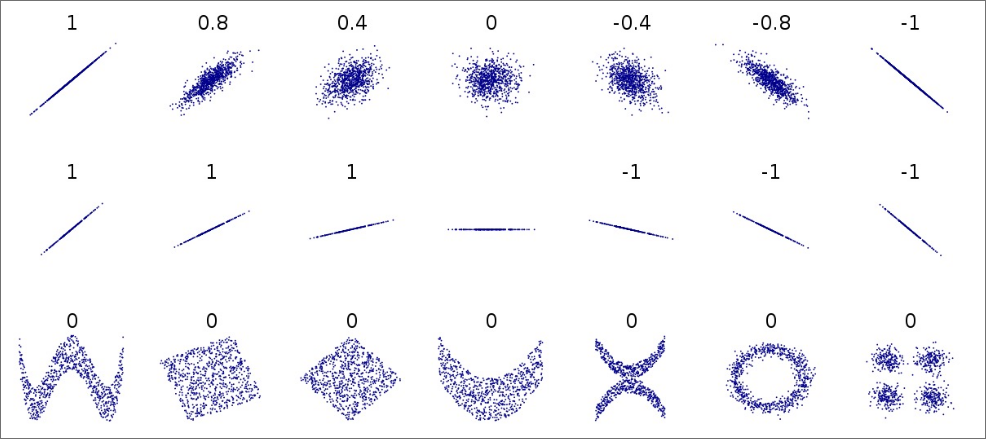
\includegraphics[scale=0.25]{2022-10-27:09:11:27.png}\newline
\begin{itemize}
\item \textcolor{orange}{The correlation is 1 if \textbf{m is positive}, and \textbf{E is 0}.}
\item \textcolor{orange}{The correlation then gradually gets less if there is a deviation between x and y.}
\item \textcolor{orange}{If \textbf{m is negative} and \textbf{E is 0}, then we have -1 correlation. This is still correlation, just negative!}
\item \textcolor{orange}{Should either x or y be constant then calculating the correlation is not possible.}
\item \textcolor{orange}{Lastly, nonsense / nonfunction data, we have correlation 0.}
\vspace{-3mm}
\end{itemize}\\
\hline
Multivariate Linear Regression & 
\textcolor{orange}{This tries to map multiple x data to y -> for example both amount of cats and the amount of dogs correlated to weather, same nonsense, but not 2 times!}\newline
Formula: \( \hat{y}_i = m_{cat} * x_i + m_{dog} * x_i + d \)\newline
\textcolor{teal}{As you can see there is no difference between this formula and the last, other than the fact that we now have two slopes.}\\
\hline
Basic Idea of Gradient Descent & 
\textbf{\textcolor{purple}{You calculate the multivariate linear regression in each step and reduce the error by modifying the parameters in each step}}\newline
\textcolor{orange}{Note that each point represents its own mode, meaning there are different parameters for each point.\newline
This is also how machine learning is done, you might have values like speed and angle that need to be changed in each iteration to take an apex in the perfect manner.}\\
\hline
Gradient Descent & 
\textcolor{orange}{We learned with Least squares that we can take the slope/intercept and see where it is equal to 0 in order to get the best fitting slope or intercept. \newline
However, \textbf{not all function will have a derivate equal to 0 -> min or max}. Also it is quite cumbersome to calculate each slope until we get to 0. It \textbf{might take thousands of steps} until we arrive where we want to be.}\newline
\textcolor{red}{INSTEAD: with gradient descent, we choose a \textbf{Learning Rate}, which will determine our \textbf{step size} in order to skip the part, where we are far away from the optimal 0.\newline
As soon as we approach derivate 0, we take smaller and smaller steps, until we can't improve the value anymore, either we are at 0 now, or 0 is not reachable and we have reached the nearest possible value instead.}\newline
\textcolor{purple}{But where do we take these 2 values from? The \textbf{Learning Rate is a user choice}, while the \textbf{step size is the previous derivate * the learning rate}.}\newline
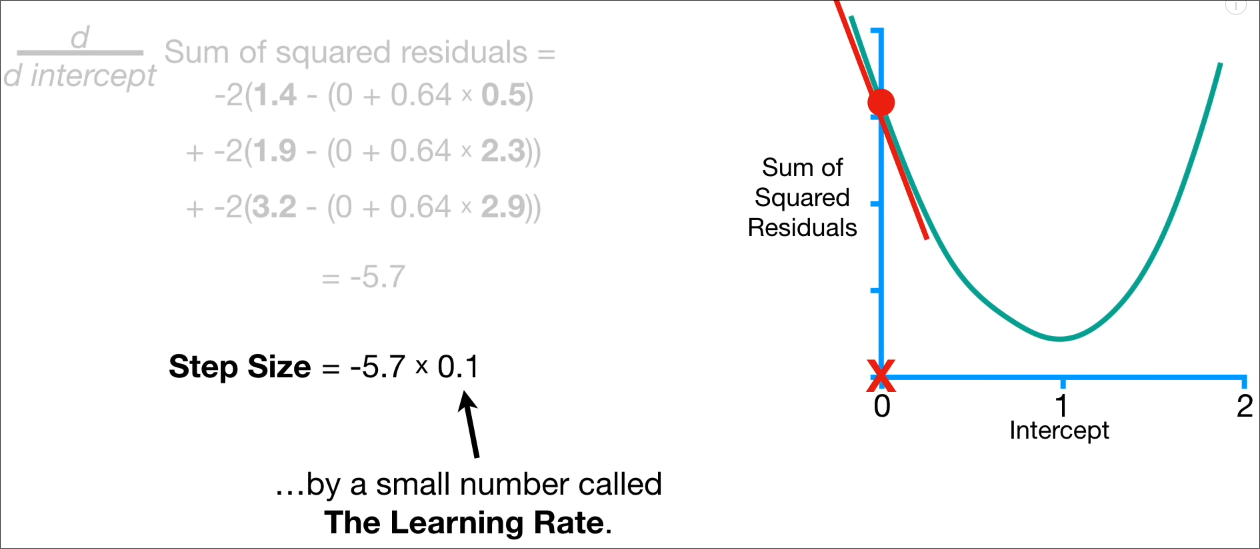
\includegraphics[scale=0.2]{2022-11-10:05:04:33.png}\newline
\textcolor{orange}{Note, the -5.7 is the derivate, therefore we multiply it with the learning rate, which is 0.1 and then we have the next step size.\newline
We can then \textbf{apply the stepsize to the slope or intercept}, whichever we want to calculate.\newline
Then we simply redo this until the derivate will be 0 or close to 0!}\newline
Small notes: Gradient descent usually \textbf{stops when the step size is smaller than the learning rate}\newline
The learning rate is \textbf{usually reduced with each step}.\newline
Also, there is usually a maximum amount of steps that gradient descent will try, for example 1000 steps.\newline
\textcolor{red}{Gradient Descent does \textbf{both intercept and slope at once!} This is also why it is called Gradient descent, because each parameter is a Gradient.}\\
\hline
\textbf{Sochastic Gradient Descent (SGD)} &
The first difference between Gradient Descent and Sochastic Gradient Descent, is that with the second we \textbf{only take random samples of data}.\newline
This allows us to reduce the number of calculations significantly. This is because each iteration of Descent needs the entire MSE to be calculated.\newline
\textbf{Calculating the MSE around random samples of data instead of the full data, decreases calculation time SIGNFICANTLY!}\newline
\textcolor{orange}{2. Difference}\newline
Sochastic Gradient Descent is usually done either with \textbf{just one point per Gradient Descent step}, or with a \textbf{mini-batch -> a small subset of data}, \newline
usually the \textbf{the best way to go is with a mini-batch, as it combines the best of both worlds}.\newline
Also, guess what, another performance increase as you need fewer calculations again!\\
\hline
\end{tabular}
\end{table}
\begin{table}[ht!]
\begin{tabular}{|m{0.2\linewidth}|m{0.755\linewidth}|}
\hline
Annealed SGD & 
\textcolor{black}{The obvious consequence of the \textbf{learning rate} is that \textbf{the learning effect decays over time,}}\textcolor{red}{this is called \textbf{annealing}.}\newline
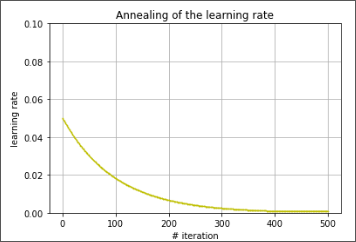
\includegraphics[scale=0.4]{2022-11-04-01:43:27.png}\\
\hline
Limitations & 
\textcolor{purple}{The limitations of this method is that you only use 1 datum -> 1 batch of datapoints for each model. This means that you will have to calculate this over, and over, and over again.\newline
\textbf{In the industry this is usually done in batches of size 32,64,128!}}\newline
\textcolor{orange}{Also, in order to use the SGD the loss function needs to be a \textbf{differentiable function}, this simply means that you can take the derivative of this function at \textbf{every point}. }\newline
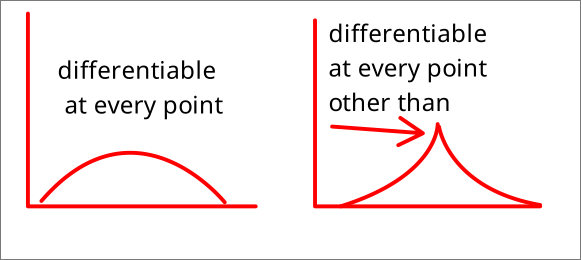
\includegraphics[scale=0.4]{2022-11-04-01:56:28.png}\newline
\textcolor{orange}{On the right side there is the top point where you have 2 interpretations of a derivation, this of course can't be done, so here you would need to define the point manually, or simply use a different function in the first place.}\\
\hline
Generalization Error & 
\textcolor{orange}{This is similar to the correlation but not causation issue. \newline
For example you might have some data that indicates that x is in linear correlation with y, but as soon as you cross a certain threshold, x behaves in an exponential correlation with y.\newline
If you only have the data for the linear part, then you will have a very, very scewed model that \textbf{will not actually represent the real world.}\newline
We call this problem the \textbf{Generalization Error}, where we generalize something without sufficient data.}\\
\hline
Training Error & 
\textcolor{orange}{When you try to fit a model to the data that you have, then you will always have to deal with the problem of potential \textbf{"noisy" data}, it essentially means inaccurate data.\newline
Should you try to perfectly fit a model with this data, then you will likely not achieve a good model as the data is as said not accurate.}\newline
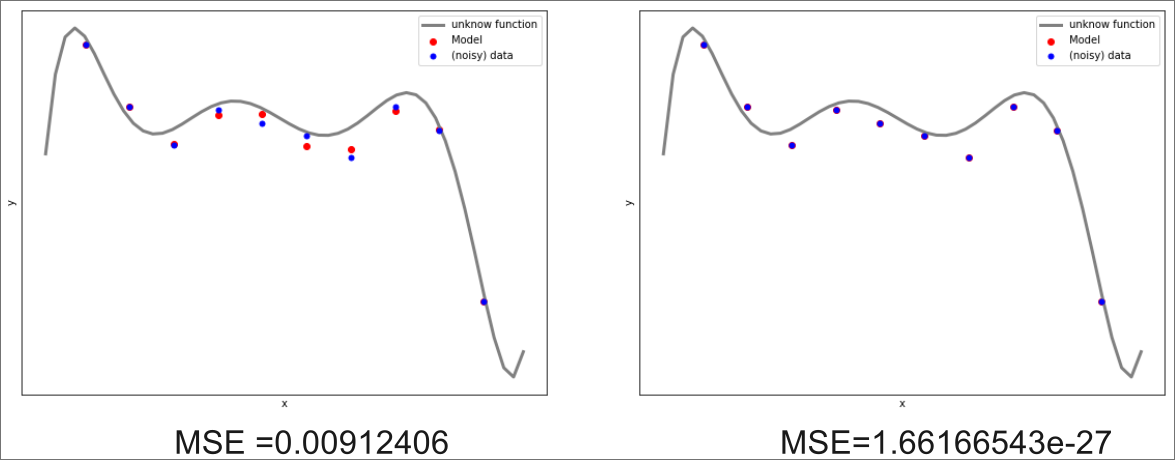
\includegraphics[scale=0.35]{2022-11-10:09:09:47.png}\newline
\textcolor{purple}{As you can see in the image, the left model with less MSE is actually the more accurate model!}\\
\hline
Reducing Generalization Error and Trainign Error with more data & 
\textcolor{orange}{The easiest way is to simply get more data before making a model, this reduces the chance that the samples are error prone, and it also reduces the chance that you will walk into the problem of generalization as you have a lot of data by now.\newline
Problem is that this is not always possible, as data collection can sometimes be very costly, or even impossible.}\\
\hline
Proper Fitting Methodology & 
\textcolor{orange}{Since we have to deal with the generalization error, it is best to \textbf{split the data into 2 sections:}}\newline
\begin{itemize}
\item \textcolor{purple}{80\% of the data for training}
\item \textcolor{purple}{20\% of the data for predictions}
\end{itemize} 
\, \newline
\textcolor{orange}{This means that after we got a model, we can see if it predicts the 20\% of the data. \newline
This way we can limit the generalization error to a certain degree.\newline
\textbf{The data for each split is chosen randomly!}}\\
\hline
Simple models vs Comlex models &
\textcolor{orange}{In comparison to complex models, \textbf{simpler models} have \textbf{a bigger training error} and a \textbf{smaller generalization error}}\newline
Or in a different language, \textbf{smaller models have the chance to underfit}, while the \textbf{complex models have the chance to overfit}\\
\hline
\end{tabular}
\end{table}
\pagebreak
\begin{table}[ht!]
\begin{tabular}{|m{0.2\linewidth}|m{0.755\linewidth}|}
\hline
Bias-Variance & 
\textcolor{orange}{This is the combination that makes up the generalization error, \newline
\textbf{bias indicates a preference towards a certain model}\newline
\textbf{variance indicates the spread of the data}}\newline
\textcolor{purple}{\textbf{A simple model for example has low variance and high bias.}}\newline
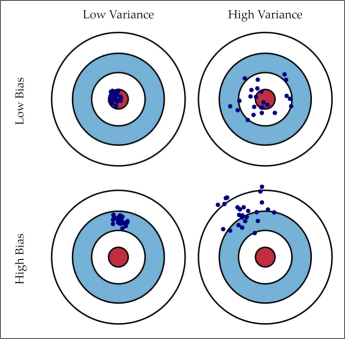
\includegraphics[scale=0.4]{2022-11-10:09:27:19.png}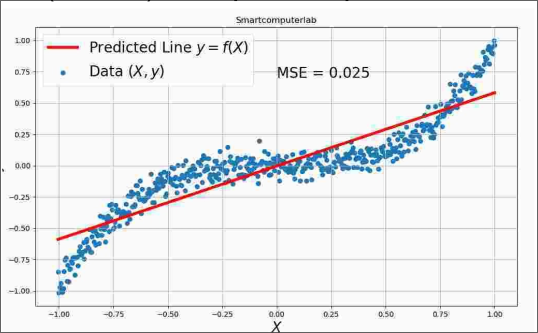
\includegraphics[scale=0.4]{2022-11-10:09:30:46.png}\\
\hline
Goal of Bias and Variance & 
\textcolor{orange}{In the end we want to have the cake and eat it too, aka we want \textbf{low Variance} and \textbf{low Bias}, \newline
the problem is that a complex model gives us low bias, but also gives high variance, while simple models give low variance but high bias.}\\
\hline
Regularization & 
\textcolor{orange}{In order to try to achieve low variance and low bias we introduce another function: \textbf{cost function for training/optimization}\newline
This means we now have 2 functions, the MSE and the optimization function.}\newline
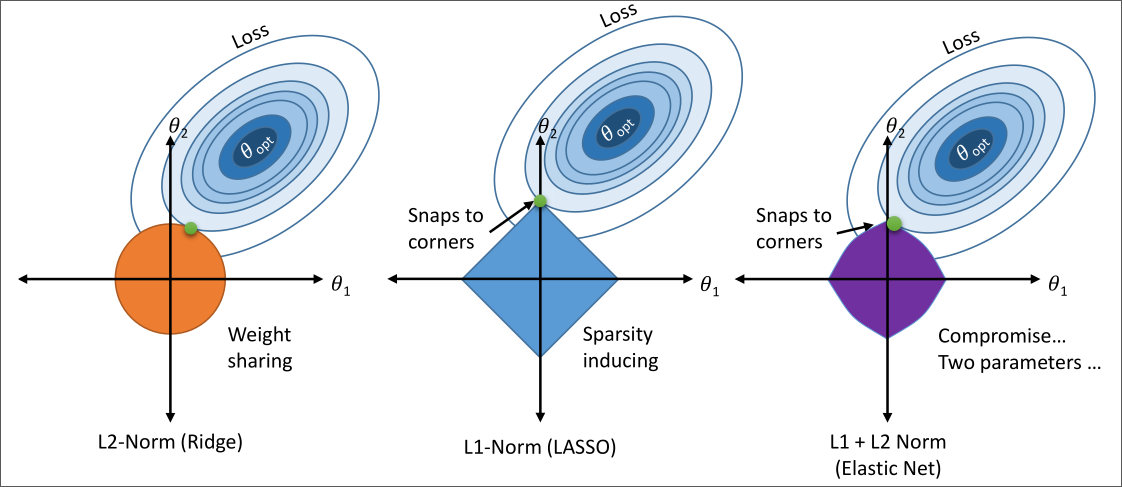
\includegraphics[scale=0.35]{2022-11-10:09:43:03.png}\newline
Regularization tries to introduce a way to \textbf{avoid underfitting or overfitting to the training data}. \newline
This means that we will need to modify our MSE to not do either of these problematic behaviors.\newline
\textbf{Rigde Regularization achieves this by taking the sum of the "corrected paramters by the MSE"}, for example you might have slope and intercept in linear regression, this means that you will have to calculate the \textbf{optimization loss function}, which is the sum of squares of each parameter multiplied by a positive number hat you choose -> \(\lambda\). \newline You then add this function to the base MSE and you have successfully implemted Ridge Regularization:\newline
\, \newline
\textcolor{OliveGreen}{Ridge Regularization:}\newline
\huge \textcolor{red}{\( \text{Ridge MSE} = \dfrac{1}{2N}\sum^{N}_{j=1}(y_j - h(w,x_j))^2 + \lambda \sum^{P}_{i=1} w_i^2 \)}\newline
\normalsize \, \newline 
\, \newline
\textcolor{OliveGreen}{Lasso Regularization:}\newline
\huge \textcolor{red}{\( \text{Lasso MSE} = \dfrac{1}{2N}\sum^{N}_{j=1}(y_j - h(w,x_j))^2 + \lambda \sum^{P}_{i=1} |w_i| \)}\newline
\normalsize \, \newline  
Legend: \newline
\begin{itemize}
\item \textcolor{Orange}{N = sum of datapoints}
\item \textcolor{Orange}{P = sum of parameters}
\item \textcolor{Orange}{w = parameter -> can be multiple ones}
\item \textcolor{Orange}{h = fitting function for example (m * x + d) for linear regression}
\item \textcolor{Orange}{\( \lambda \) = positive number chosen by user 0 to infinity}
\vspace{-3mm}
\end{itemize}\\
\hline
Difference between lasso regularization and ridge regularization & 
\textbf{Lasso regularization can hit the slope 0, while ridge is very unlikely to hit it.}\\
\hline

\hline

\hline

\hline

\hline
\end{tabular}
\end{table}
\end{document}
